\documentclass[12pt]{article}
\usepackage[utf8]{inputenc}
\usepackage[T1]{fontenc}
\usepackage[spanish,es-lcroman]{babel}
\usepackage{amsmath}
\usepackage{amsthm}
\usepackage{physics}
\usepackage{tikz}
\usepackage{float}
\usepackage{cancel}
\usepackage[autostyle,spanish=mexican]{csquotes}
\usepackage[per-mode=symbol]{siunitx}
\usepackage{gensymb}
\usepackage{multicol}
\usepackage{enumitem}
\usepackage{stackengine}
\usepackage{stix}
\usepackage[left=2.00cm, right=2.00cm, top=2.00cm, 
     bottom=2.00cm]{geometry}

\usepackage{Estilos/ColoresLatex}
\usepackage{makecell}
\usepackage{wrapfig}
% \usepackage{titlesec}
\usetikzlibrary{angles,quotes}
\newcommand{\sectionbreak}{\clearpage}

\newcommand{\textocolor}[2]{\textbf{\textcolor{#1}{#2}}}
%\renewcommand{\questionlabel}{\thequestion)}

\newcommand{\Cancel}[2][black]{{\color{#1}\cancel{\color{black}#2}}}

\newcommand\deci[1]{%
    \kern-.4ex\stackunder[0.4pt]{$#1$}{$\color{blue}\acwunderarcarrow$}
}

\newcommand\decposl[1]{%    <--- Decimal position to left
    \kern-.4ex\stackunder[0.4pt]{$#1$}{%
      \reflectbox{$\color{red}\kern-.6ex\acwunderarcarrow$}
      }
}

\decimalpoint
\sisetup{bracket-numbers = false}

\title{\vspace*{-2cm} Guía de estudio Movimiento Circular}
\author{M. en C. Ramón Gustavo Contreras Mayén \\ {\fontsize{14}{14}\selectfont Universidad del Valle de México. Campus San Rafael}}
% \institute{Universidad del Valle de México. Campus San Rafael.}
\date{}

\begin{document}
\maketitle

\section{El círculo y la circunferencia.}
\subsection{Elementos.}

Para un mejor entendimiento del movimiento circular se requiere el manejo de distintos elementos de la circunferencia y del círculo, a continuación se mencionan los que trabajaremos en el tema.

\begin{enumerate}
\item La circunferencia se define como una curva plana, cerrada, cuyos puntos son equidistantes de otro, el centro, situado en el mismo plano.
\begin{figure}[H]
    \centering
    \begin{tikzpicture}
        \draw [line width=2pt] (0,0) circle (2.3cm);
        % \draw [line width=2pt] (0,0)-- (1.882349956410611,1.3216499693946844);
        \draw [fill=black] (0,0) circle (0.5pt);
        \draw [fill] (0, 0) circle (0.05cm);
    \end{tikzpicture}    
\end{figure}
\item Se define como el círculo al área o superficie plana contenida dentro de una circunferencia, en la imagen que se muestra a continuación, el área se presenta de color gris.
\begin{figure}[H]
    \centering
    \begin{tikzpicture}
        \draw [line width=1pt,fill=black,fill opacity=0.32] (0,0) circle (2.3cm);
    \end{tikzpicture}
\end{figure}
\item El centro del círculo es el punto que está a la misma distancia de todos los puntos pertenecientes a la circunferencia.
\begin{figure}[H]
    \centering
    \begin{tikzpicture}
        \draw [line width=2pt] (3,2) circle (2.2840315234251913cm);
        \draw [fill=black] (3,2) circle (1pt);
        \draw[color=black] (3.22,2.35) node {$C$};
    \end{tikzpicture}
\end{figure}
\item El radio es un segmento de recta que une el centro con cualquier punto perteneciente a la circunferencia.
\begin{figure}[H]
    \centering
    \begin{tikzpicture}
        \draw [line width=2pt] (3,2) circle (2.2840315234251913cm);
        \draw [line width=2pt,color=red] (3,2)-- (4.963935340498931,0.8339133915787598);
        \draw (3.7,2.46) node[anchor=north west] {r};
        \draw [fill=black] (3,2) circle (1pt);
        \draw [fill=black] (4.963935340498931,0.8339133915787598) circle (1pt);
    \end{tikzpicture}
\end{figure}
\item El arco es un segmento de la circunferencia delimitado por dos puntos de la misma, en la figura que se muestra, el segmento de color azul es el arco.
\begin{figure}[H]
    \centering
    \begin{tikzpicture}
        \draw [line width=1.2pt] (0,0) circle (2cm);
        \draw [shift={(0,0)},line width=2pt,color=ao]  plot[domain=3.141592653589793:5.395207291363843,variable=\t]({1*2*cos(\t r)+0*2*sin(\t r)},{0*2*cos(\t r)+1*2*sin(\t r)});
        \draw [fill=black] (0,0) circle (1pt);
        \draw [fill=black] (-2,0) circle (1pt);
        \draw [fill=black] (1.2619639312733133,-1.5515949974671883) circle (1pt);
    \end{tikzpicture}
\end{figure}
\item La cuerda es un segmento de recta que une dos puntos cualquiera de una circunferencia.
\begin{figure}[H]
    \centering
    \begin{tikzpicture}
        \draw [line width=2pt] (3,2) circle (2.2840315234251913cm);
        \draw [line width=2pt,color=ao] (0.8476698966091152,2.764378915222931)-- (4.7757163258948765,3.4365345557801246);
        \draw [fill=black] (0.8476698966091152,2.764378915222931) circle (1pt);
        \draw [fill=black] (4.7757163258948765,3.4365345557801246) circle (1pt);
    \end{tikzpicture}
\end{figure}
\item El diámetro es la mayor cuerda  de una circunferencia. Hay infinitos diámetros y todos pasan por el centro de la circunferencia.
\begin{figure}[H]
    \centering
    \begin{tikzpicture}[scale=0.8]
        \draw [line width=2pt] (3,2) circle (2.2840315234251913cm);
        \draw [line width=2pt,color=darkgreen] (0.7301778625231852,1.7456233811448398)-- (5.267958315569716,2.27049044130648);
        \draw (2.54,2.94) node[anchor=north west] {d};
        \draw [fill=black] (3,2) circle (1pt);
    \end{tikzpicture}
\end{figure}
\item La recta secante, es una recta que corta dos puntos cualesquiera de una circunferencia.
\begin{figure}[H]
    \centering
    \begin{tikzpicture}[scale=0.8]
        \draw [line width=2pt] (3,2) circle (2.2840315234251913cm);
        \draw [line width=2pt,color=darkmagenta] (0.74,4.04)-- (3.3,-1);
        \draw [fill=black] (3,2) circle (1pt);
    \end{tikzpicture}
\end{figure}
\item La recta tangente, es una recta que toca a la circunferencia en un solo punto y es perpendicular al radio.
\begin{figure}[H]
    \centering
    \begin{tikzpicture}[scale=0.75]
        \draw [line width=2pt] (3,2) circle (2.2840315234251913cm);
        \draw [line width=2pt,color=auburn] (3.02,5)-- (6.12,2.38);
        \draw [fill=black] (3,2) circle (1pt);
        \draw [fill=black] (4.469516826105958,3.774924488903997) circle (1pt);
    \end{tikzpicture}
\end{figure}
\end{enumerate}

\section{Movimiento uniformemente acelerado.}

\subsection{El movimiento circular.}

Un objeto describe un movimiento circular cuando su trayectoria es una circunferencia. En este movimiento el vector velocidad varía constantemente de dirección, y su magnitud puede variar o permanecer constante.

Por tanto, en un movimiento circular un cuerpo se puede mover con rapidez constante o no, pero su aceleración formará siempre un ángulo recto (\ang{90}) con su velocidad y se desplazará formando un círculo.
    
La aceleración que recibe el cuerpo está dirigida hacia el centro del círculo y recibe el nombre de aceleración normal, radial o centrípeta.

\subsection{Conceptos.}

\begin{enumerate}
\item \textit{Ángulo}: Es la abertura comprendida entre dos radios cualesquiera, que limitan un arco de circunferencia.
\item \textit{Radián}: Es el ángulo central al que corresponde un arco de longitud igual al radio.
\begin{figure}[H]
\centering
\begin{tikzpicture}
    \def\R{1.7}
    \def\ang{55}
    \coordinate (O) at (0,0);
    \coordinate (X) at (\R,0);
    \coordinate (R) at (\ang:\R);
    %\draw[vector] (O) -- (R) node[midway,right=4,above left=0] {$\vb{r}$};
    \draw [dashed] (O) -- (X) node[midway,below right=0] {$r$};
    \draw [dashed] (O) -- (R) node[midway,right=4,above left=0] {$r$};
    % \draw pic[->,"$\Delta\theta$",draw=black,angle radius=20,angle eccentricity=1.5] {angle=X--O--R};
    \draw (O) circle (\R);
    % \draw[red!80!black,very thick,line cap=round] (X) arc (0:\ang:\R) node[midway,above right=-2] {$\Delta s$};
    \draw [red!80!black,very thick,line cap=round] (X) arc (0:\ang:\R);
    \draw (0.5, 0) arc(0:55:0.5);
    \draw (0.8, 0.3) node {$\theta$};
    %\draw[dashed] (R) -- ({\R*cos(\ang)},0);
    %\draw[dashed] (R) -- (0,{\R*sin(\ang)});
    \end{tikzpicture}
\end{figure}
Para obtener el valor en radianes de un ángulo que se mide en grados, ocupamos la siguiente relación:
\begin{align*}
\ang{360} = 2 \, \pi \unit{\radian}
\end{align*}
En donde planteamos una regla de tres para obtener ya sea un valor de grados a radianes, o de radianes a grados.
\item \textit{Vector de posición}: Si observamos el movimiento de un objeto colocado encima de un disco que gira, podemos precisar su posición si tomamos como origen del sistema de referencia al centro de la trayectoria circular.

De esta forma, el vector que nos indicará su posición para cada intervalo de tiempo se encontrará determinado por el radio de la circunferencia, mismo que permanece constante.

Por tanto, el vector de posición tendrá una magnitud constante y su dirección será la misma que tenga el radio de la circunferencia. Cuando el objeto colocado sobre un disco que se desplace, su cambio de posición se podrá expresar mediante desplazamientos del vector de posición, lo cual dará lugar a desplazamientos angulares.
\item \textit{Desplazamiento angular}: Por tanto, el desplazamiento angular es la magnitud física que cuantifica la magnitud de la rotación que experimenta un objeto de acuerdo con su ángulo de giro.

El desplazamiento angular se representa por la letra griega $\theta$ (theta),  sus unidades de medida son: 
\begin{enumerate}
\item El radián cuando el sistema usado es el internacional. [\unit{\radian}]
\item En grados sexagesimales. [${}^{\circ}$]
\item Revoluciones (pueden indicarse por minuto [rpm] o por segundo [rps])
\end{enumerate}
\begin{figure}[H]
    \centering
    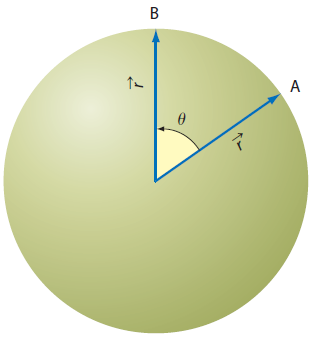
\includegraphics[scale=0.75]{Imagenes/Movimiento_Circular_01.png}
    \caption{Se presenta un desplazamiento angular.}
\end{figure}
Si el objeto realizar distintos desplazamientos angulares, podemos verlo en la siguiente figura:
\begin{figure}[H]
    \centering
    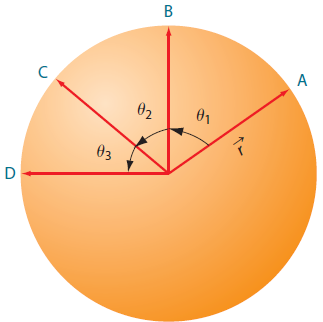
\includegraphics[scale=0.75]{Imagenes/Movimiento_Circular_02.png}
    \caption{Un objeto realizando distintos desplazamientos angulares.}
\end{figure}
El objeto se desplazó del punto $A$ al $B$ con un desplazamiento angular $\theta_{1}$, luego hizo otro desplazamiento angular $\theta_{2}$ que lo dejó en la posición $C$, por último, para llegar al punto $D$ hizo un desplazamiento angular $\theta_{3}$.
\end{enumerate}    
    
\subsection{Conceptos adicionales.}

Para tener un contexto completo sobre el movimiento circular, se requieren de manera adicional los siguientes conceptos:
\begin{enumerate}
\item \textit{El periodo}: Es el tiempo que tarda un objeto en dar una vuelta completa o en completar un ciclo. En el sistema internacional de unidades (SIU), la unidad del periodo es el segundo.
\begin{align*}
T = \dfrac{\text{segundos transcurridos}}{\text{1 ciclo}} \hspace{1cm} \text{Unidades} \rightarrow \left[ \unit{\second} \right]
\end{align*}
\item \textit{La frecuencia}: Es el número de vueltas, revoluciones o ciclos que efectúa un móvil en un segundo.
\begin{align*}
f = \dfrac{\text{número de ciclos}}{\text{1 segundo}} \hspace{1cm} \text{Unidades} \rightarrow \left[ \dfrac{1}{\unit{\second}} = \si{\hertz} \right]
\end{align*}
Las unidades de la frecuencia es el Hertz.
\end{enumerate}
    
\section{Dinámica circular.}

\subsection{Velocidad angular.}

La magnitud de la velocidad angular representa el cociente entre la magnitud del desplazamiento angular de un objeto y el tiempo que tarda en efectuarlo:

\begin{align*}
\omega = \dfrac{\theta}{t} \hspace{1cm} \left[ \dfrac{\text{rad}}{\unit{\second}} \right]
\end{align*}
donde:
\begin{enumerate}[label=\alph*)]
\item $\omega$ es la magnitud de la velocidad angular.
\item $\theta$ es la magnitud del desplazamiento angular.
\item $t$ es el tiempo en que se efectúa el desplazamiento.
\end{enumerate}

La magnitud de la velocidad angular se puede expresar en función de los cambios en su desplazamiento angular con respecto al cambio en el tiempo, de la siguiente forma:
\begin{eqnarray*}
\begin{aligned}
\omega = \dfrac{\Delta \theta}{\Delta t} =  \dfrac{\theta_{2} - \theta_{1}}{t_{2} - t_{1}}
\end{aligned}
\end{eqnarray*}

La magnitud de la velocidad angular también se puede determinar si se conoce su periodo $(T)$ es decir, el tiempo que tarda en dar una vuelta completa o una revolución:
\begin{align*}
\ang{360}  = 2 \, \pi \, \text{radianes}
\end{align*}
La expresión que se utiliza es:
\begin{eqnarray*}
\begin{aligned}
\omega = \dfrac{2 \, \pi \, \text{rad}}{T} =  \dfrac{2 \, \pi}{T} \hspace{1cm} \left[ \dfrac{\text{rad}}{\unit{\second}} \right]
\end{aligned}
\end{eqnarray*}
Pero como $T = 1 / f$, la velocidad angular se determina también por:
\begin{align*}
\omega = 2 \, \pi \, f \hspace{1cm} \left[ \dfrac{\text{rad}}{\unit{\second}} \right]
\end{align*}

\subsection{Velocidad angular media.}

Cuando la velocidad angular de un objeto no es constante o uniforme, podemos determinar la magnitud de la velocidad angular media al conocer las magnitudes de la velocidad angular inicial y su velocidad angular final:
\begin{align*}
\omega_{m} = \dfrac{\omega_{f} + \omega_{i}}{2}
\end{align*}
donde:
\begin{enumerate}[label=\roman*)]
\item $\omega_{m}$ es la magnitud de la velocidad angular.
\item $\omega_{f}$ es la magnitud de la velocidad angular final.
\item $\omega_{0}$ es la magnitud de la velocidad angular inicial.
\end{enumerate}

\subsection{Velocidad lineal o tangencial.}

Cuando un objeto se encuentra girando,  cada una de las partículas del mismo se mueve a lo largo de la circunferencia descrita por él con una velocidad lineal cuya magnitud será mayor, a medida que aumenta el radio de la circunferencia.

Esta velocidad lineal también recibe el nombre de velocidad tangencial, porque la dirección de la velocidad siempre es tangente a la circunferencia recorrida por la partícula. Representa la magnitud de la velocidad que llevaría ésta si saliera disparada tangencialmente.
\begin{figure}[H]
    \centering
    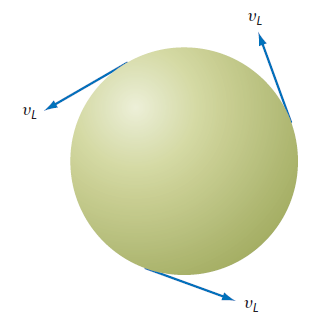
\includegraphics[scale=0.75]{Imagenes/Movimiento_Circular_03.png}
\end{figure}

Para calcular la magnitud de la velocidad tangencial o lineal se usa la ecuación:
\begin{align*}
v_{L} = \dfrac{2 \, \pi \, r}{T}
\end{align*}
donde:
\begin{enumerate}[label=\alph*)]
\item $r$ es el radio de la circunferencia en metros.
\item $T$ es el periodo en segundos.
\item $v_{L}$ es la velocidad lineal en \unit{\meter\per\second}
\end{enumerate}

Como la velocidad angular es $\omega = 2 \, \pi /T$, la magnitud de la velocidad lineal se expresa también como:
\begin{align*}
v_{L} = \omega \cdot r
\end{align*}

\subsection{Ejercicios.}

\begin{enumerate}
\item Ejercicio 1.

¿Cuál es la magnitud de la velocidad angular de una llanta de un camión que gira desplazándose \SI{12}{\radian} en \SI{0.5}{\second}?

\vspace*{0.5cm}
\begin{minipage}[t]{0.4\linewidth}
\textbf{Datos:}
\begin{align*}
\theta &= \SI{12}{\radian} \\
t &= \SI{0.5}{\second} \\
\omega &= \, ?
\end{align*}
\end{minipage}
\begin{minipage}[t]{0.4\linewidth}
\textbf{Expresión:}
\begin{align*}
\omega = \dfrac{\theta}{t}
\end{align*}
\end{minipage}

\textbf{Sustitución:}
\begin{align*}
\omega = \dfrac{\SI{12}{\radian}}{\SI{0.5}{\second}} = \SI[per-mode=fraction]{24}{\radian\per\second}
\end{align*}
\item Ejercicio 2.

Determina la magnitud de la velocidad angular y la frecuencia de una pelota atada a un hilo, si gira con un periodo de \SI{0.6}{\second}.

\vspace*{0.5cm}
\begin{minipage}[t]{0.4\linewidth}
\textbf{Datos:}
\begin{align*}
T &= \SI{0.6}{\second} \\
\omega &= \, ? \\
f &= \, ?
\end{align*}
\end{minipage}
\begin{minipage}[t]{0.4\linewidth}
\textbf{Expresiones:}
\begin{align*}
\omega &= \dfrac{2 \, \pi \, \unit{\radian}}{T} \\[0.5em]
f &= \dfrac{1}{T}
\end{align*}
\end{minipage}

\textbf{Sustitución:}
\begin{align*}
\omega &= \dfrac{2 \, \pi \, \unit{\radian}}{\SI{0.6}{\second}} = \dfrac{\SI{6.2832}{\radian}}{\SI{0.6}{\second}} = \SI[per-mode=fraction]{10.47}{\radian\per\second} \\[0.5em]
f &= \dfrac{1}{\SI{0.6}{\second}} = \SI{1.66}{\hertz}
\end{align*}
\item Ejercicio 3.

Halla la magnitud de la velocidad angular y el periodo de una rueda que gira con una frecuencia de \num{430} revoluciones por minuto.

Como se nos indica que la frecuencia $f = 430 \, \text{rpm}$, hay que obtener el valor correspondiente en segundos.
\begin{align*}
f = 430 \, \dfrac{\text{rev}}{\unit{\minute}} \left( \dfrac{\SI{1}{\minute}}{\SI{60}{\second}} \right) = \SI{7.16}{\hertz}
\end{align*}

\vspace*{0.5cm}
\begin{minipage}[t]{0.4\linewidth}
\textbf{Datos:}
\begin{align*}
f &= \num{430} \, \text{rpm} = \SI{7.16}{\hertz} \\
\omega &= \, ? \\
T &= \, ?
\end{align*}
\end{minipage}
\begin{minipage}[t]{0.4\linewidth}
\textbf{Expresiones:}
\begin{align*}
\omega &= \dfrac{2 \, \pi \, f \, \unit{\radian}}{T} \\[0.5em]
f &= \dfrac{1}{T}
\end{align*}
\end{minipage}

\textbf{Sustitución:}
\begin{align*}
\omega &= 2 \, \pi \, \left( \SI{7.16}{\hertz} \right) \, \unit{\radian}= \SI[per-mode=fraction]{45.02}{\radian\per\second} \\[0.5em]
T &= \dfrac{1}{\SI{7.16}{\hertz}} = \SI{0.139}{\second}
\end{align*}
\item Ejercicio 4.

Calcular la magnitud de la velocidad lineal de una partícula cuyo radio de giro es de \SI{25}{\centi\meter} y tiene un periodo de \SI{0.01}{\second}.

\vspace*{0.5cm}
\begin{minipage}[t]{0.4\linewidth}
\textbf{Datos:}
\begin{align*}
r &= \SI{25}{\centi\meter} = \SI{0.25}{\meter} \\
T &= \SI{0.01}{\second} \\
v_{T} &= \, ?
\end{align*}
\end{minipage}
\begin{minipage}[t]{0.4\linewidth}
\textbf{Expresiones:}
\begin{align*}
v_{T} &= \dfrac{2 \, \pi \, r }{T}
\end{align*}
\end{minipage}

\textbf{Sustitución:}
\begin{align*}
v_{T} &= \dfrac{2 \, \pi \, \left( \SI{0.25}{\meter} \right)}{\SI{0.01}{\second}}= \SI[per-mode=fraction]{157.07}{\meter\per\second}
\end{align*}
\end{enumerate}

\section{Movimiento Circular Uniformemente Acelerado.}
\subsection{Aceleración angular.}

El movimiento circular uniformemente acelerado (MCUA) se presenta cuando un móvil con trayectoria circular aumenta o disminuye en cada unidad de tiempo la magnitud de su velocidad angular en forma constante. Por lo que la magnitud de su aceleración angular permanece constante.

En el movimiento circular vamos a ocupar la letra griega $\alpha$ para denotar la aceleración circular, de esta manera evitamos confusiones con la aceleración lineal que se revisó en el tema de Movimiento Uniformemente Acelerado (MUA).

\subsection{Aceleración angular media.}

Cuando durante el movimiento circular de un móvil su velocidad angular no permanece constante, sino que varía, decimos que sufre una aceleración angular. Cuando la velocidad angular varía es conveniente determinar cuál es la magnitud de su aceleración angular media, misma que se expresa de la siguiente manera:
\begin{align*}
\alpha = \dfrac{\omega_{f} - \omega_{i}}{t_{f} - t_{i}} \hspace{1cm} \text{Unidades} \rightarrow \left[ \unit[per-mode=fraction]{\radian\per\square\second} \right]
\end{align*}

\subsection{Aceleración centrípeta.}

La aceleración centrípeta $(a_{C})$ es la aceleración experimentada por un objeto que se mueve en una trayectoria curvilínea, como una circunferencia.

Esta aceleración siempre está dirigida hacia el centro de la trayectoria circular  y es perpendicular a la velocidad tangencial $(v_{T})$ del objeto en cualquier punto dado de la trayectoria.
\begin{figure}[H]
    \centering
\begin{tikzpicture}
    \draw (0, 0) circle (2cm);
    \draw [-stealth, thick] (2, 0) -- (0.5, 0) node [midway, above] {$a_{c}$}; 
    \draw [-stealth, thick] (2, 0) -- (2, 2.5) node [midway, right] {$v_{T}$}; 
\end{tikzpicture}
\end{figure}

La magnitud de la aceleración centrípeta $(a_{c})$ se calcula utilizando la siguiente fórmula:
\begin{align*}
a_{c} = \dfrac{v_{T}^{2}}{r} \hspace{1cm} \left[ \unit[per-mode=fraction]{\meter\per\square\second} \right]
\end{align*}
donde:
\begin{enumerate}[label=\alph*)]
\item $v_{T}$ es la velocidad lineal del objeto.
\item $r$ es el radio de la trayectoria circular.
\end{enumerate}

\subsection{Ecuaciones MCUA.}

Las ecuaciones empleadas para el MCUA son las mismas que se utilizan para el MRUA con las siguientes variantes.

\begin{enumerate}[label=\roman*)]
\item En lugar de magnitud del desplazamiento en metros hablaremos de magnitud del desplazamiento angular en radianes ($\theta$ en lugar de d).
\item La magnitud de la velocidad en \unit{\meter\per\second} será sustituida por la magnitud de la velocidad angular en \unit{\radian\per\second} ($\omega$ en lugar de $v$).
\item La magnitud de la aceleración en \unit{\meter\per\square\second} se cambiará por la magnitud de la aceleración angular en \unit{\radian\per\square\second} ($\alpha$ en lugar de a)
\end{enumerate}

\subsection{Desplazamientos angulares.}

Las siguientes expresiones nos permiten obtener el desplazamiento angular $\theta$, que se reporta en radianes:
\begin{eqnarray*}
\begin{aligned}
\theta &= \omega_{0} \, t + \dfrac{\alpha \, t^{2}}{2} \\[0.5em] 
\theta &= \dfrac{\omega_{f}^{2} - \omega_{0}^{2}}{2 \, \alpha} \\[0.5em] 
\theta &= \dfrac{\omega_{f} + \omega_{0}}{2} \, t
\end{aligned}
\end{eqnarray*}
Si el objeto parte del reposo su velocidad angular inicial $(\omega_{0})$ es cero, y las tres ecuaciones anteriores se reducen a:
\begin{eqnarray*}
\begin{aligned}
\theta &= \dfrac{\alpha \, t^{2}}{2} \\[0.5em] 
\theta &= \dfrac{\omega_{f}^{2}}{2 \, \alpha} \\[0.5em] 
\theta &= \dfrac{\omega_{f}}{2} \, t
\end{aligned}
\end{eqnarray*}

Para calcular la magnitud de las velocidades angulares finales:
\begin{eqnarray*}
\begin{aligned}
\omega_{f} &= \omega_{0} + \alpha \, t \\[0.5em] 
\omega_{f} &= \omega_{0}^{2} + 2 \, \alpha \, \theta
\end{aligned}
\end{eqnarray*}

Si el objeto parte del reposo su velocidad inicial $(\omega_{0})$ es cero, y las dos ecuaciones anteriores se reducen a:
\begin{eqnarray*}
\begin{aligned}
\omega_{f} &= \alpha \, t \\[0.5em] 
\omega_{f} &= 2 \, \alpha \, \theta
\end{aligned}
\end{eqnarray*}

\subsection{Ejercicios.}

\begin{enumerate}
\item Ejercicio 1.

En una pista circular de radio \SI{100}{\meter}, un auto le da dos vueltas en cada minuto.
\begin{enumerate}[label=\roman*)]
\item ¿Cuál es el periodo del movimiento del auto?
\item ¿Cuál es la distancia que recorre en cada ciclo?
\item ¿Qué valor tiene la velocidad lineal del vehículo?
\item ¿Cuánto vale su aceleración centrípeta?
\item ¿Cuál es su velocidad angular?
\end{enumerate}

Para resolver el ejercicio, hay que tomar en cuenta que el auto da dos vueltas en un minuto a la pista circular, este valor representa la frecuencia (número de ciclos en un segundo), por lo que hay que expresar la frecuencia en segundos:
\begin{align*}
f = 2 \, \dfrac{\text{rev}}{\unit{\minute}} \left( \dfrac{\SI{1}{\minute}}{\SI{60}{\second}} \right) = \SI{0.033}{\hertz}
\end{align*}
Para responder el inciso ii) que nos pide el valor de la distancia que recorre el auto alrededor de la pista circular, hay que tomar en cuenta que nos piden el valor del perímetro de la circunferencia, que recuperamos ocupando el valor del radio:
\begin{align*}
d = 2 \, \pi \, r
\end{align*}
\vspace*{0.5cm}
\begin{minipage}[t]{0.4\linewidth}
\textbf{Datos:}
\begin{align*}
r &= \SI{100}{\meter} \\
f &= 2 \, \text{rpm} = \SI{0.033}{\hertz} \\
T &= \, ? \\
d &= \, ? \\
v_{T} &= \, ? \\
a_{C} &= \, ? \\
\omega &= \, ?
\end{align*}
\end{minipage}
\begin{minipage}[t]{0.4\linewidth}
\textbf{Expresiones:}
\begin{align*}
T &= \dfrac{1}{f} \\
d &= 2 \, \pi \,  r \\
v_{T} &= \dfrac{2 \, \pi \, r }{T} \\
a_{C} &= \dfrac{(v_{t})^{2}}{r} \\
\omega &= \dfrac{2 \, \pi \, \unit{\radian}}{T}
\end{align*}
\end{minipage}

\textbf{Sustitución:}

Inciso i):
\begin{align*}
T = \dfrac{1}{\SI{0.033}{\hertz}} = \SI{30}{\second}
\end{align*}
Inciso ii):
\begin{align*}
d = 2 \, \pi \left( \SI{100}{\meter} \right) = \SI{628.31}{\meter}
\end{align*}
Inciso iii):
\begin{align*}
v_{T} = \dfrac{2 \, \pi (\SI{100}{\meter})}{\SI{30}{\second}} = \dfrac{\SI{628.31}{\meter}}{\SI{30}{\second}} = \SI[per-mode=fraction]{20.94}{\meter\per\second}
\end{align*}
inciso iv):
\begin{align*}
a_{C} = \dfrac{\displaystyle \left( \SI[per-mode=fraction]{20.94}{\meter\per\second} \right)^{2}}{\SI{100}{\meter}} = \dfrac{\displaystyle \SI[per-mode=fraction]{438.48}{\square\meter\per\square\second}}{\SI{100}{\meter}} = \SI[per-mode=fraction]{4.38}{\meter\per\square\second}
\end{align*}
inciso v):
\begin{align*}
\omega = \dfrac{2 \, \pi \, \unit{\radian}}{\SI{30}{\second}} = \SI[per-mode=fraction]{0.2094}{\radian\per\second}
\end{align*}


\item Ejercicio 2.

Una polea motriz de \SI{6}{\centi\meter} de diámetro se hace girar a 9 rev/s.
\begin{enumerate}[label=\alph*)]
\item ¿Cuál sería la velocidad lineal de una banda accionada por la polea?
\item ¿Cuál es la aceleración centrípeta en un punto localizado en el borde de la polea?
\end{enumerate}

Para obtener la velocidad lineal, ahora ocuparemos la expresión que la relaciona con la frecuencia de giro de la polea.

\vspace*{0.5cm}
\begin{minipage}[t]{0.4\linewidth}
\textbf{Datos:}
\begin{align*}
d &= \SI{6}{\centi\meter} = \SI{0.06}{\meter} \\
\hspace{0.2cm} \Rightarrow \hspace{0.2cm} r &= \SI{0.03}{\meter} \\
f &= 9 \, \text{rps} = \SI{9}{\hertz} \\
v_{T} &= \, ? \\
a_{C} &= \, ? \\
\omega &= \, ?
\end{align*}
\end{minipage}
\begin{minipage}[t]{0.4\linewidth}
\textbf{Expresiones:}
\begin{align*}
\omega &= 2 \, \pi \, f \\
v_{T} &= \omega \, r \\
a_{C} &= \dfrac{(v_{t})^{2}}{r}
\end{align*}
\end{minipage}

\textbf{Sustitución:}

inciso i) 
\begin{align*}
\omega &= 2 \, \pi \, \left( \SI{9}{\hertz} \right) \unit{\radian} = \SI[per-mode=fraction]{56.54}{\radian\per\second} \\[0.5em]
v_{T} &= \left( \SI[per-mode=fraction]{56.54}{\radian\per\second} \right) (\SI{0.03}{\meter}) = \SI[per-mode=fraction]{1.69}{\meter\per\second} \\[0.5em]
a_{C} &= \dfrac{\displaystyle \left( \SI[per-mode=fraction]{1.69}{\meter\per\second} \right)^{2}}{\SI{0.03}{\meter}} = \dfrac{\displaystyle \SI[per-mode=fraction]{2.85}{\square\meter\per\square\second}}{\SI{0.03}{\meter}} = \SI[per-mode=fraction]{95.20}{\meter\per\square\second}
\end{align*}


\item Ejercicio 3.

Un objeto está atado a una cuerda y se mueve en un círculo horizontal de \SI{90}{\centi\meter} de radio. Sin considerar los efectos de la gravedad y supóngamos que el objeto gira con una frecuencia de 80 rpm.

Determina la velocidad lineal $(v_{T})$ y la aceleración centrípeta $(a_{c})$.

\vspace*{0.5cm}
\begin{minipage}[t]{0.4\linewidth}
\textbf{Datos:}
\begin{align*}
r &= \SI{90}{\centi\meter} = \SI{0.9}{\meter} \\
f &= 80 \, \text{rpm} = 1.33 \, \text{rps} \\
f &= \SI{1.33}{\hertz} \\
v_{T} &= \, ? \\
a_{C} &= \, ? \\
\end{align*}
\end{minipage}
\begin{minipage}[t]{0.4\linewidth}
\textbf{Expresiones:}
\begin{align*}
\omega &= 2 \, \pi \, f \\
v_{T} &= \omega \, r \\
a_{C} &= \dfrac{(v_{t})^{2}}{r}
\end{align*}
\end{minipage}

\textbf{Sustitución:}

Hay que ocupar la expresión para obtener la velocidad angular y con ella, obtener primero la velocidad tangencial:
\begin{align*}
    \omega &= 2 \, \pi \, \left( \SI{1.33}{\hertz} \right) \unit{\radian} = \SI[per-mode=fraction]{8.35}{\radian\per\second} \\[0.5em]
    v_{T} &= \left( \SI[per-mode=fraction]{8.35}{\radian\per\second} \right) (\SI{0.9}{\meter}) = \SI[per-mode=fraction]{7.52}{\meter\per\second} \\[0.5em]
    a_{C} &= \dfrac{\displaystyle \left( \SI[per-mode=fraction]{7.52}{\meter\per\second} \right)^{2}}{\SI{0.9}{\meter}} = \dfrac{\displaystyle \SI[per-mode=fraction]{56.56}{\square\meter\per\square\second}}{\SI{0.9}{\meter}} = \SI[per-mode=fraction]{62.85}{\meter\per\square\second}
    \end{align*}

\item Ejercicio 4.

Un ventilador gira dando $120$ vueltas en \SI{1}{\minute}, si la longitud de cada aspa es de \SI{30}{\centi\meter}, y al apagarse se detiene después de \SI{80}{\second}:
\begin{enumerate}[label=\roman*)]
\item ¿Cuál es su aceleración angular?
\item ¿Cuál es la aceleración centrípeta de un punto a la mitad del aspa?
\end{enumerate}


Consideraciones. El enunciado nos dice que:
\begin{enumerate}
\item El ventilador se apaga y se detiene, es decir, deja de girar luego de \SI{80}{\second}, por lo que su velocidad angular final $(\omega_{f})$ vale cero.
\item El aspa mide de largo \SI{30}{\centi\meter}, entendiendo que va del centro del ventilador al extremo, es decir, la longitud del aspa a partir del centro corresponde al radio.
\end{enumerate}

\vspace*{0.5cm}
\begin{minipage}[t]{0.4\linewidth}
\textbf{Datos:}
\begin{align*}
f &= 120 \, \text{rpm} = 2 \, \text{rps} = \SI{2}{\hertz} \\
r &= \SI{30}{\centi\meter} = \SI{0.3}{\meter} \\
\Rightarrow \hspace{0.2cm} r &= \SI{15}{\centi\meter} = \SI{0.15}{\meter} \\
t &= \SI{80}{\second} \\
\omega_{f} &= 0 \\
\alpha &= \, ? \\
a_{C} &= \, ? \\
\end{align*}
\end{minipage}
\begin{minipage}[t]{0.4\linewidth}
\textbf{Expresiones:}
\begin{align*}
\omega &= 2 \, \pi \, f \\[0.5em]
\alpha &= \dfrac{\omega_{f} - \omega_{0}}{t} \\[0.5em]
v_{T} &= \omega \, r \\[0.5em]
a_{C} &= \dfrac{(v_{t})^{2}}{r}
\end{align*}
\end{minipage}
\end{enumerate}

Sustitución:

inciso i):

Un punto en la mitad del aspa, está ubicado en la mitad del radio: \SI{0.15}{\meter}.
\begin{align*}
\omega &= 2 \, \pi \, \left( \SI{2}{\hertz} \right) \, \unit{\radian} = \SI[per-mode=fraction]{12.56}{\radian\per\second} \\
\alpha &= \dfrac{ \displaystyle0 - \SI[per-mode=fraction]{12.56}{\radian\per\second}}{\SI{80}{\second}} = - \SI[per-mode=fraction]{0.157}{\radian\per\square\second}
\end{align*}
El signo negativo de la aceleración angular $(\alpha)$ nos indica que las aspas del ventilador se están desacelerando. 

\vspace*{0.5cm}
inciso ii):
\begin{align*}
a_{c} = \dfrac{\displaystyle \left( \SI[per-mode=fraction]{12.56}{\radian\per\second} \right)^{2}}{\SI{0.15}{\meter}} = \dfrac{\displaystyle \SI[per-mode=fraction]{157.75}{\square\meter\per\square\second}}{\SI{0.15}{\meter}} = \SI[per-mode=fraction]{1051.69}{\meter\per\square\second}
\end{align*}
\end{document}